\documentclass[]{article}


%-----------------------------------------------------------------------------------------------------------------------------------------
%
%   GLOBALS
%
%-----------------------------------------------------------------------------------------------------------------------------------------
\newcommand{\DOCTITLE}{

}
\newcommand{\DOCAUTHOR}{

}
\newcommand{\DISCLAIMER}
{
    \topskip0pt
    \vspace*{\fill}
    {
    \centering
        \small{
            THIS DOCUMENT IS INTENDED FOR INTERNAL USE ONLY
        }
    }
    \\
    {
    \centering
        \small{
        UNAUTHORIZED DISTRIBUTION OF THIS DOCUMENT IS STRICTLY PROHIBITED 
        }
    }
    \vspace*{\fill}
}

\usepackage{lmodern}
\usepackage{amssymb,amsmath}
\usepackage{ifxetex,ifluatex}
\usepackage{fixltx2e} % provides \textsubscript
\ifnum 0\ifxetex 1\fi\ifluatex 1\fi=0 % if pdftex
  \usepackage[T1]{fontenc}
  \usepackage[utf8]{inputenc}
\else % if luatex or xelatex
  \ifxetex
    \usepackage{mathspec}
    \usepackage{xltxtra,xunicode}
  \else
    \usepackage{fontspec}
  \fi
  \defaultfontfeatures{Mapping=tex-text,Scale=MatchLowercase}
  \newcommand{\euro}{€}
\fi
% use upquote if available, for straight quotes in verbatim environments
\IfFileExists{upquote.sty}{\usepackage{upquote}}{}
% use microtype if available
\IfFileExists{microtype.sty}{%
\usepackage{microtype}
\UseMicrotypeSet[protrusion]{basicmath} % disable protrusion for tt fonts
}{}
\ifxetex
  \usepackage[setpagesize=false, % page size defined by xetex
              unicode=false, % unicode breaks when used with xetex
              xetex]{hyperref}
\else
  \usepackage[unicode=true]{hyperref}
\fi
\usepackage[usenames,dvipsnames]{color}
\hypersetup{breaklinks=true,
            bookmarks=true,
            pdfauthor={},
            pdftitle={Engineering Simulator for Rocket Flight Analysis},
            colorlinks=true,
            citecolor=blue,
            urlcolor=blue,
            linkcolor=magenta,
            pdfborder={0 0 0}}
\urlstyle{same}  % don't use monospace font for urls
\usepackage{graphicx,grffile}
\makeatletter
\def\maxwidth{\ifdim\Gin@nat@width>\linewidth\linewidth\else\Gin@nat@width\fi}
\def\maxheight{\ifdim\Gin@nat@height>\textheight\textheight\else\Gin@nat@height\fi}
\makeatother
% Scale images if necessary, so that they will not overflow the page
% margins by default, and it is still possible to overwrite the defaults
% using explicit options in \includegraphics[width, height, ...]{}
\setkeys{Gin}{width=\maxwidth,height=\maxheight,keepaspectratio}
\usepackage[normalem]{ulem}
% avoid problems with \sout in headers with hyperref:
\pdfstringdefDisableCommands{\renewcommand{\sout}{}}
\setlength{\parindent}{0pt}
\setlength{\parskip}{6pt plus 2pt minus 1pt}
\setlength{\emergencystretch}{3em}  % prevent overfull lines
\providecommand{\tightlist}{%
  \setlength{\itemsep}{0pt}\setlength{\parskip}{0pt}}
\setcounter{secnumdepth}{0}

\title{Engineering Simulator for Rocket Flight Analysis}
\date{}

% Redefines (sub)paragraphs to behave more like sections
\ifx\paragraph\undefined\else
\let\oldparagraph\paragraph
\renewcommand{\paragraph}[1]{\oldparagraph{#1}\mbox{}}
\fi
\ifx\subparagraph\undefined\else
\let\oldsubparagraph\subparagraph
\renewcommand{\subparagraph}[1]{\oldsubparagraph{#1}\mbox{}}
\fi

%-----------------------------------------------------------------------------------------------------------------------------------------
%
%   PAGE SIZE AND MARGINS
%
%-----------------------------------------------------------------------------------------------------------------------------------------
\usepackage[a4paper,headheight=30pt]{geometry}
%\usepackage[letterpaper, portrait, margin=2in]{geometry}
\addtolength{\topmargin}{-.5in}
\addtolength{\textheight}{1.75in}

\usepackage{graphicx}

\usepackage{fancyhdr}
\pagestyle{fancy}


%-----------------------------------------------------------------------------------------------------------------------------------------
% Page break after sections
%-----------------------------------------------------------------------------------------------------------------------------------------
%\usepackage{titlesec}
%\newcommand{\sectionbreak}{\clearpage}

\lhead{
    %left header content
%    \topskip0pt
%    \vspace*{\fill}
    {
    \centering
        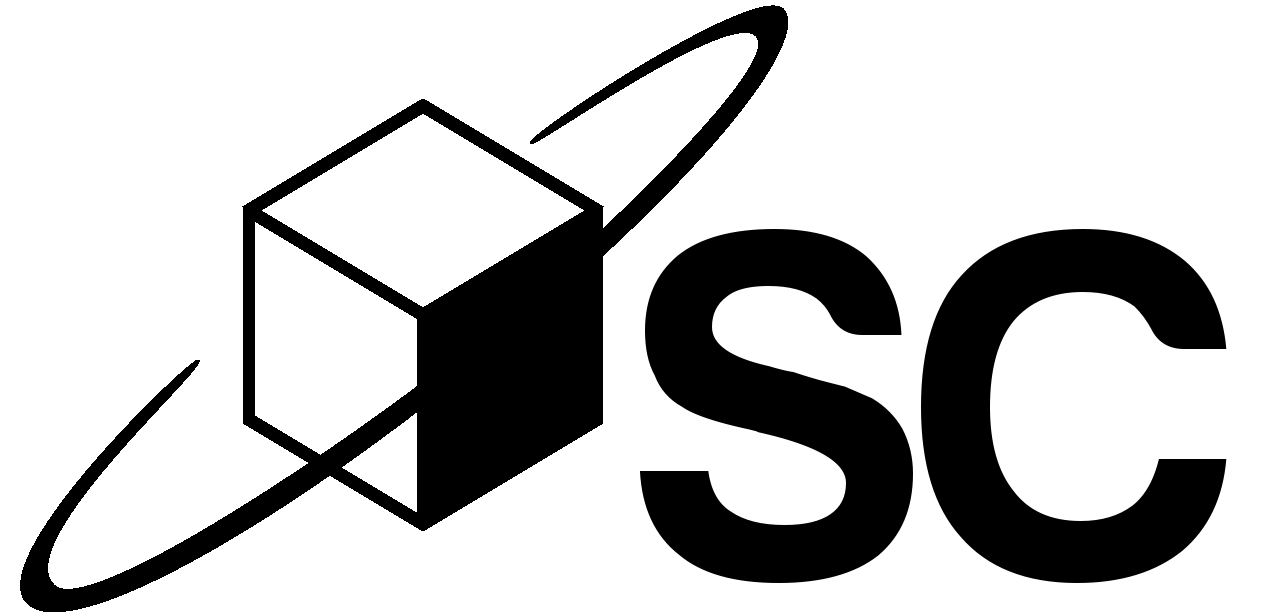
\includegraphics[height=2.66em]{template/sc.png}
    }
%    \vspace*{\fill}
}
\chead{
    \topskip0pt
    \vspace*{\fill}
    {
    \centering
        \small{
            THIS DOCUMENT IS INTENDED FOR INTERNAL USE ONLY
        }
    }
    \\
    {
    \centering
        \small{
        UNAUTHORIZED DISTRIBUTION OF THIS DOCUMENT IS STRICTLY PROHIBITED 
        }
    }
    \vspace*{\fill}
}
\rhead{
%    \topskip0pt
%    \vspace*{\fill}
    % right header content
    {
    \centering
        
\includegraphics[height=3.25em]{template/scrd.png}
    }
%    \vspace*{\fill}
}
\lfoot{
    % left footer content
    \topskip0pt
    \vspace*{\fill}
    SCRD
    Revision 0.1
    \vspace*{\fill}
}
\cfoot{
    % middle footer content
    \topskip0pt
    \vspace*{\fill}
    {
    \centering
    SCRD Internal Documents Template \\
    \today
    }
    \vspace*{\fill}
}
\rfoot{
    % right footer content
    \topskip0pt
    \vspace*{\fill}
    \thepage
    \vspace*{\fill}
}
% extend the header into the margins
\usepackage{calc}
\fancyheadoffset[L,R]{\marginparsep+\marginparwidth}

%--------------------------------------------------------------------------------------------------------------
%	My Packages
%--------------------------------------------------------------------------------------------------------------
\usepackage{capt-of}

%--------------------------------------------------------------------------------------------------------------
%	
%	COPY FRONTMATTER AND MAINMATTER AND BACKMATTER COMMANDS
%	
%--------------------------------------------------------------------------------------------------------------
\makeatletter

\newcommand\frontmatter{%
    \cleardoublepage
  %\@mainmatterfalse
  \pagenumbering{roman}}

\newcommand\mainmatter{%
    \cleardoublepage
 % \@mainmattertrue
  \pagenumbering{arabic}}

\newcommand\backmatter{%
  \if@openright
    \cleardoublepage
  \else
    \clearpage
  \fi
 % \@mainmatterfalse
   }

\makeatother

%--------------------------------------------------------------------------------------------------------------
%
%	BEGIN DOCUMENT
%
%--------------------------------------------------------------------------------------------------------------
\begin{document}

%\maketitle

%--------------------------------------------------------------------------------------------------------------
%
%	TITLE PAGE
%
%--------------------------------------------------------------------------------------------------------------
\begin{titlepage}

\newcommand{\HRule}{\rule{\linewidth}{0.5mm}} % Defines a new command for the horizontal lines, change thickness here

\center % Center everything on the page
 
%----------------------------------------------------------------------------------------
%	HEADING SECTIONS
%----------------------------------------------------------------------------------------

\includegraphics[width=200pt,height=200pt]{../images/rocketry_logo_large.png}\\[1cm] % Include a department/university logo - this will require the graphicx package
\textsc{\Large Space Concordia - Rocketry Division}\\[0.5cm] % Major heading such as course name
\textsc{\large Aurelius CR-2-4G - Structural Team}\\[0.5cm] % Minor heading such as course title

%----------------------------------------------------------------------------------------
%	LOGO SECTION
%----------------------------------------------------------------------------------------

\begin{figure}[ht]
    \centering
    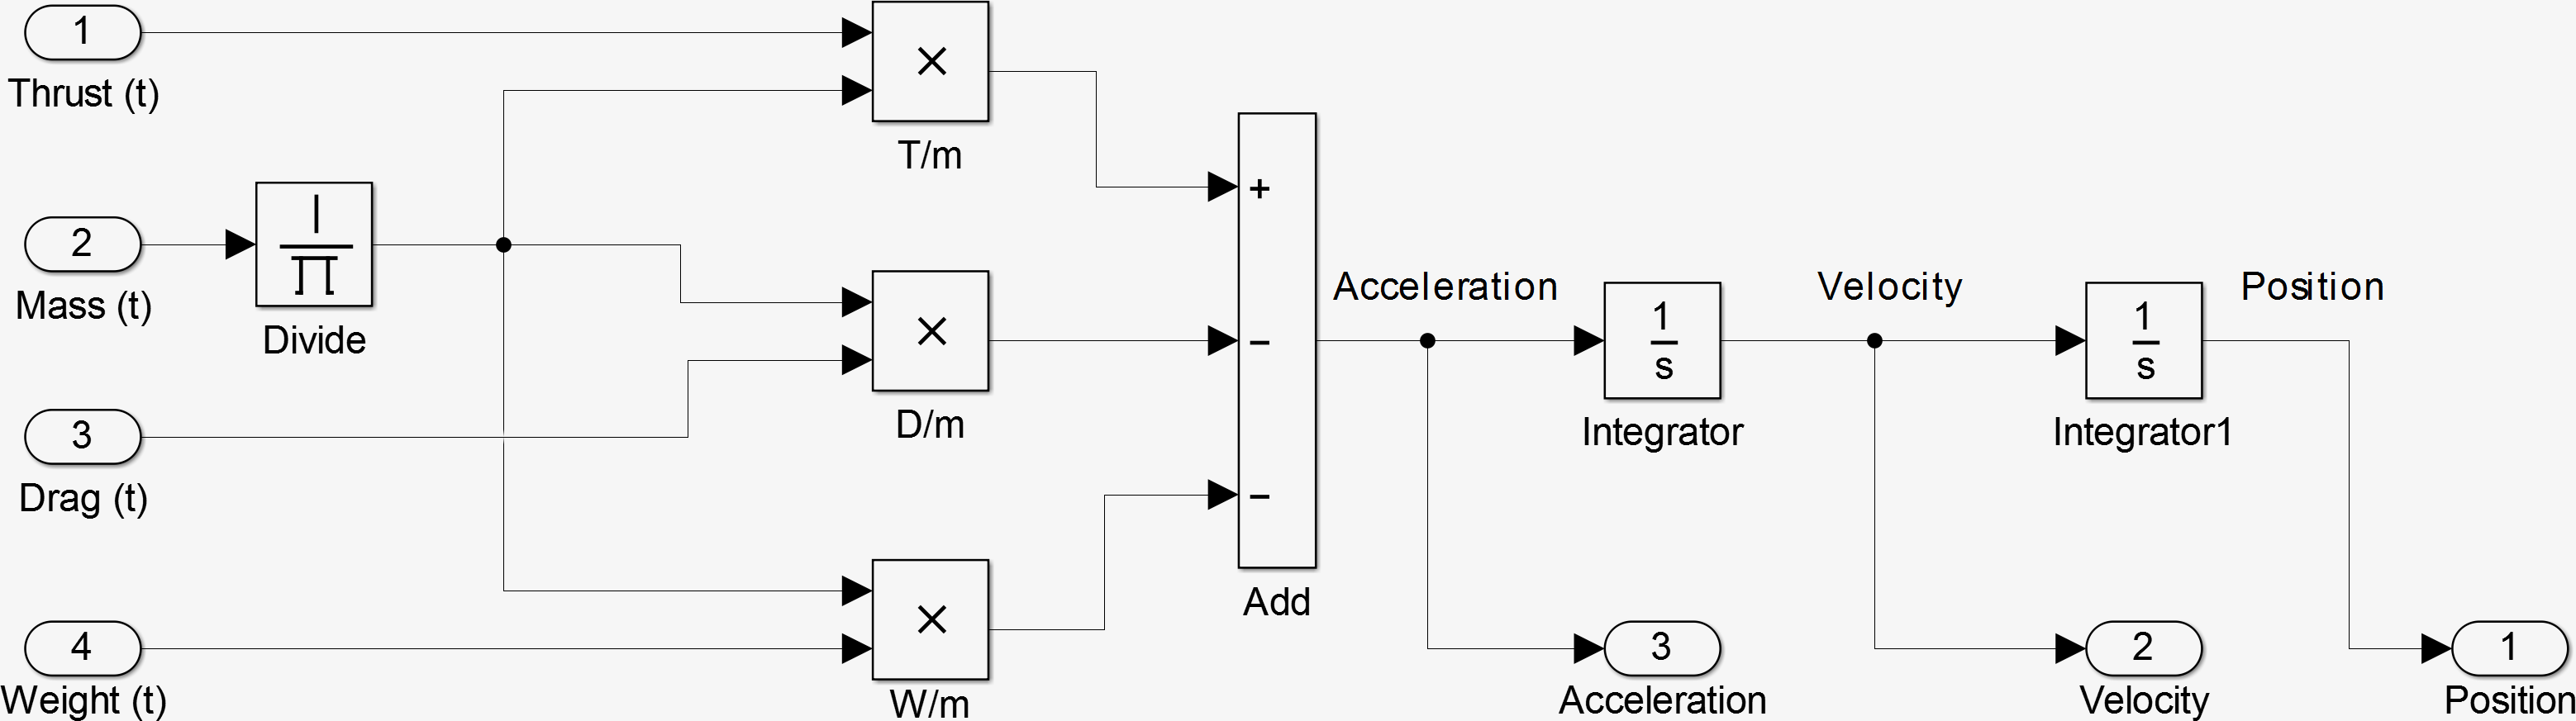
\includegraphics[height=100pt]{../images/vertical_model_simplified.png}\\
\end{figure}

%----------------------------------------------------------------------------------------
%	TITLE SECTION
%----------------------------------------------------------------------------------------

\HRule \\[0.6cm]
{ \Huge \bfseries 
Engineering Simulation for Rocket Flight Analysis
}\\[0.4cm] 

\HRule \\[1cm]
 
%----------------------------------------------------------------------------------------
%	AUTHOR SECTION
%----------------------------------------------------------------------------------------

\begin{minipage}{0.4\textwidth}
\begin{flushleft} \large
	\begin{tabular} {r l} 
        \emph{Author(s):} & Shawn Bulger	\\
	\end{tabular}
\end{flushleft}
\end{minipage}
~
\begin{minipage}{0.4\textwidth}
\begin{flushright} \large
	\begin{tabular} {r l} 
		\emph{Coordinator:} & Dr. Ashok Kaushal 		\\
		\emph{Supervisor:}  & Dr. Mehdi Hojjati 		\\
		\emph{EIR:}         & Dominic Ng  		        \\
	\end{tabular}
\end{flushright}
\end{minipage}\\[2cm]

%----------------------------------------------------------------------------------------
%	DATE SECTION
%----------------------------------------------------------------------------------------

{\large \today}\\[2cm] % Date, change the \today to a set date if you want to be precise

\vfill % Fill the rest of the page with whitespace

\end{titlepage}


%--------------------------------------------------------------------------------------------------------------
%
%	FRONT MATTER
%
%--------------------------------------------------------------------------------------------------------------
\frontmatter

%\section*{Abstract}
\begin{abstract}
A team from the Space Concordia association at Concordia University is
entering a submission into the International Rocket Engineering
Competition run by the Experimental Sounding Rocket Association (ESRA).
To complement the team's mechanical design process, an Engineering
Simulation is required to validate the flight performance criteria set
by the competition. Matlab Simulink was used as an environment to model
the flight dynamics and output the results. Thorough unit and
integration testing was performed, in addition to comparison with
experimental data to validate the model. Significant areas beyond the
scope of the project are explored, such as a thorough stability
analysis, preliminary considerations of a 6DOF simulator based on
quaternion rotations, stochastic parameter variation to determine
simulation uncertainties, and a generally in-depth review of literature
and theory relating to high-powered rocket flight. The primary flight
performance criteria of the CR\_2-4G rocket was confirmed to comply with
all competition requirements and suggests the rocket is on course to
maximize the team scores for performance. Future considerations are
recommended for improvement and extension of the simulator.
\end{abstract}
\clearpage

{
\hypersetup{linkcolor=black}
\setcounter{tocdepth}{3}
\tableofcontents
\clearpage
}


\listoftables
\listoffigures
\clearpage

%--------------------------------------------------------------------------------------------------------------
%
%	MAIN MATTER
%
%--------------------------------------------------------------------------------------------------------------
\mainmatter

%--------------------------------------------------------------------------------------------------------------
% body
%--------------------------------------------------------------------------------------------------------------
\section{Rigid-Body Rotation (Pitch, Yaw) Stability
Analysis}\label{rigid-body-rotation-pitch-yaw-stability-analysis}

\subsection{Overview}\label{overview}

Due to disturbances such as wind, and imperfections and imbalances in
the construction, the rocket will tend to fly at an \emph{Angle of
Attack} into the free stream, wherein the velocity vector (taken from
the \emph{Center of Gravity}) is not parallel with the longitudinal
axis. This will cause non-linear changes to the magnitude of the
aerodynamic forces, which, as a further simplification, can be said to
be acting on the \emph{Center of Pressure}. In order for the aerodynamic
forces to straighten the rocket in its forward motion, and to stabilize
the oscillatory rotation about the COG, the COP must be located behind
the COG.

The moment arm about the COG is the distance of the COP from the tip of
the nose cone, minus the distance of the COG from the tip of the nose
cone. Then, the sum of forces at the COP is the \emph{Restoring Force}
(\(F_R\)) minus the \emph{Damping Force} (\(F_D\)), and the sum of the
Moments about the COG is expressed as follows.

The \emph{Moment} of a rigid body about its COG can be expressed as the
product of the \emph{Moment of Inertia} of the rigid body and the
\emph{Angular acceleration} of the body.

\begin{equation}
\label{eq_moment}
M = I \lambda 
\end{equation}

\begin{itemize}
\tightlist
\item
  \(\lambda\) is the \emph{angular acceleration} of the rigid body,
  which is the second time derivative of the angular displacement
\end{itemize}

\[ 
\lambda = \ddot{\alpha}
\] \[
\omega = \dot{\alpha}
\]

\begin{itemize}
\tightlist
\item
  \(\omega\) is the \emph{angular velocity}, which is the first time
  derivative of the angular displacement
\item
  \(\alpha\) is the \emph{angle of attack}
\end{itemize}

\subsection{Longitudinal Static Stability
Margin}\label{longitudinal-static-stability-margin}

The \emph{Longitudinal Static Stability Margin} (\(S_{lm}\)) is the
distance between the \emph{Center of Gravity} and the \emph{Center of
Pressure} divided by the outer diameter of the body tube when the rocket
is positioned at an angle-of-attack (\(\alpha\)) of zero {[}1{]}.

\[ S_{lm} = \dfrac{COP - COG}{OD} \]

When traveling under a non-zero angle of attack, the Stability Margin is
adjusted using the body lift correction factor Equation
\ref{eq_coefficient_normal_force_body_lift}.

The result is dimensionless, however the ratio determined is measured in
the number of \emph{calibers}.

\begin{quote}
2a - The static stability margin falls above 2 (but less than 3)
calibers at launch
\end{quote}

\subsection{Requirement}\label{requirement}

\begin{itemize}
\tightlist
\item
  2a - The static stability margin falls above 2 (but less than 3)
  calibers at launch
\item
  2b - The dynamic stability is greater than 0 even in winds up to 8.33
  m/s
\item
  2f - The vehicle does not experience resonant pitching/yawing motion
  in flight
\end{itemize}

\subsection{Assumptions}\label{assumptions}

\begin{itemize}
\tightlist
\item
  small angle of attack (less than 10\(^\circ\))
\item
  incompressible flow
\item
  neglect viscous forces
\item
  neglect compressibility effects {[}2{]}
\item
  neglect lift force on the body tube {[}2{]}
\item
  neglect the effect of roll due to having 3 fins vs 4
\end{itemize}

\subsection{Definition of Terms}\label{definition-of-terms}

\subsubsection{Rocket Normal Force}\label{rocket-normal-force}

The \emph{Rocket Normal Force} is the resultant force applied at the
\emph{Center of Pressure} perpendicular to the longitudinal axis of the
rocket, when the rocket flies at an angle-of-attack.

\begin{equation}
\label{rocket_normal_force}
F_{N} = \dfrac{1}{2} \rho \vec{v}^2 A_{c} C_N
\end{equation}

{[}2{]}

Where \(A_c\) is the cross-sectional area of the body tube, and \(C_N\)
is the \emph{Normal Force Coefficient}, and is a function of
angle-of-attack (\(\alpha\)). The small angle approximation is applied,
wherein small angles can be approximated as a linear function of the
angle.

\begin{equation}
\label{normal_force_coefficient}
C_N = C_{N \alpha} \cdot \alpha
\end{equation}

{[}2{]}

\subsubsection{Corrective Moment
Coefficient}\label{corrective-moment-coefficient}

The \emph{Corrective Moment Coefficient} describes the reaction of the
rocket against a disturbance about its longitudinal axis.

\begin{equation}
\label{eq_coef_moment_corrective}
C_{MC} = \dfrac{1}{2} \rho \vec{v}^2 A_{ref} C_{N \alpha} (COP-COG)
\end{equation}

Where:

\begin{itemize}
\tightlist
\item
  \(\rho\) is the local density of air
\item
  \(\vec{v}\) is the velocity of the rocket
\item
  \(A_{ref}\) is the reference area of the rocket flying into the free
  stream
\item
  \(C_{N \alpha}\) is the \emph{Stability Derivative} \sout{\emph{Normal
  Force Coefficient}}
\item
  \((COP-COG)\) is the distance between the \emph{Center of Pressure}
  and \emph{Center of Gravity}
\end{itemize}

Note: a rocket with a high \emph{Corrective Moment Coefficient} is going
to weathercock faster at lower velocities.

\href{https://www.apogeerockets.com/education/downloads/Newsletter193.pdf}{Corrective
Moment Coefficient}

\paragraph{Dimensional Analysis}\label{dimensional-analysis}

\begin{equation}
\label{eq_c1_dim_anal}
\dfrac{kg}{m^3} \left[ \dfrac{m}{s} \right]^2 m^2 m = \dfrac{kg \cdot m }{s^2} \cdot m 
\end{equation}

\subsubsection{Damping Moment
Coefficient}\label{damping-moment-coefficient}

As the rocket responds to a disturbance, the \emph{Corrective Moment}
reactions forces act in an oscillating manner - weathercocking into the
wind, then turning back towards the vertical direction. In order to
reach dynamic stability, this oscillation must decay and settle to a
reasonable response. The \emph{Damping Moment Coefficient} represents
how fast the response settles towards zero.

There are two \emph{Damping Moment Coefficients} to consider, the
\emph{Aerodynamic Damping Moment Coefficient} and the \emph{Propulsive
Damping Moment Coefficient}.

Then the \emph{Damping Moment Coefficient} is the sum of the two moment
components coefficients.

\begin{equation}
\label{eq_coef_moment_damping}
C_{DM} = C_{ADM} + C_{PDM}
\end{equation}

\paragraph{Aerodynamic Damping Moment
Coefficient}\label{aerodynamic-damping-moment-coefficient}

Each rocket component contributes to the \emph{Aerodynamic Damping
Moment Coefficient}

\begin{equation}
\label{eq_coef_moment_damping_aero}
C_{ADM} = \dfrac{1}{2} \rho \vec{v} A_{ref} \sum \left( C_{N \alpha,x} \cdot \left[ COP_{x} - COG \right]^2  \right) 
\end{equation}

NOTE: Why isn't \(\vec{v}\) SQUARED? It might have something to with the
fact that the ADM is a function of angular displacement, and DM is a
function of angular velocity??

Where:

\begin{itemize}
\tightlist
\item
  \(\rho\) is the local density of air
\item
  \(\vec{v}\) is the velocity of the rocket
\item
  \(A_{ref}\) is the reference area of the rocket flying into the free
  stream
\item
  \sout{\(C_{NF,x}\)} \(C_{N \alpha}\) is the \sout{\emph{Normal Force
  Coefficient}} \emph{Stability Derivative}
\item
  \(COP_{x}\) is the distance of \emph{Center of Pressure} of the rocket
  component to the nose cone tip
\item
  \(COG\) is the distance between the rocket \emph{Center of Gravity} to
  the nose cone tip
\end{itemize}

\subparagraph{Dimensional Analysis}\label{dimensional-analysis-1}

\begin{equation}
\label{eq_c2a_dim_anal}
\dfrac{kg}{m^3} \dfrac{m}{s} m^2 m^2 = \dfrac{kg \cdot m }{s} \cdot m 
\end{equation}

\paragraph{Propulsive Damping Moment
Coefficient}\label{propulsive-damping-moment-coefficient}

Also known as \emph{Jet Damping}, as propulsion creates forward
momentum, it resists rotation of the rocket.

\begin{equation}
\label{eq_coef_moment_damping_jet}
C_{PDM} = \dot{m} \left( d_{tip,nozzle} - COG \right) ^2
\end{equation}

\subparagraph{Jet Damping - Dimensional
Analysis}\label{jet-damping---dimensional-analysis}

\[
\dot{m} \left( d_{tip,nozzle} - COG \right) ^2 :
\left[ \dfrac{kg}{s} \cdot m^2 \right]
\] \[
M = fd : 
\left[ \dfrac{kg \cdot m^2}{s^2} \right]
\]

Note: why is the \emph{Jet Damping Moment} missing a 1/t?

\href{https://www.apogeerockets.com/education/downloads/Newsletter195.pdf}{Damping
Moment Coefficient - Source}

\paragraph{Pitch Damping Moment}\label{pitch-damping-moment}

The \emph{Pitch Damping Moment} is a moment opposing the \emph{Rocket
Restoring Moment} and dampens the oscillation.

\begin{equation}
\label{eq_moment_damping_pitch}
0.55 \dfrac{l^4 r_t}{A_{ref} d} \dfrac{\omega^2}{v^2_0}
\end{equation}

According to {[}3{]}, the \emph{Pitch Damping Moment} is essentially
insignificant until near apogee. This is because it is proportional to
\(\dfrac{\omega^2}{v^2_0}\) (as seen in \ref{eq_moment_damping_pitch}),
which will be near zero until apogee due to very small angular
velocities made smaller by squaring the \(\omega\) term.

The \emph{Pitch Damping Moment} of each rocket component must be
calculated individually. For instance, the \emph{Pitch Damping Moment}
of a fin is as follows.

\begin{equation}
\label{eq_moment_damping_pitch_fin}
C_{damp} = 0.6 \dfrac{N A_{fin} d_{COP}^3}{A_{ref} d} \dfrac{\omega^2}{v^2_0}
\end{equation}

\subsection{Derivation of the Harmonic Motion
Equation}\label{derivation-of-the-harmonic-motion-equation}

Suppose a high-powered rocket is launched in quiescent air vertically,
and flies straight without wobbling. Then, suppose a small and momentary
disturbance (e.g.~a short gust of wind) is experienced on the side of
the rocket causing an angular deflection, . If the rocket is
\emph{stable}, a restoring force causes a \emph{corrective moment} which
will act in the opposite direction of the deflection. This
\emph{corrective moment} can be considered a function of angular
displacement {[}1{]}.

\begin{equation}
M_{corrective} = F (\alpha)
\end{equation}

As the rocket gains velocity in the direction opposite the disturbance,
a \emph{damping moment} is generated as a result of the relative speed
of the air, in the direction orthogonal to the longitudinal axis. As
this \emph{damping moment} opposes the angular velocity caused by the
\emph{corrective moment}, its sign is opposite to the angular velocity.
The \emph{damping moment} is also a function of angular velocity
{[}1{]}.

\begin{equation}
M_{damping} = G (\omega)
\end{equation}

Then, taking a sum of Moments, the rotation of the rocket can be
described as follows {[}1{]}

\[
I \lambda = -F(\alpha) - G(\omega) 
\] \[
I \left( \dfrac{d^2\alpha}{dt^2} \right) = -F(\alpha) - G \left(\dfrac{d\alpha}{dt} \right) 
\]

\begin{equation}
\label{eq_rocket_diff}
I \left( \dfrac{d^2\alpha}{dt^2} \right) + F(\alpha) + G \left(\dfrac{d\alpha}{dt} \right) = 0
\end{equation}

This nonlinear, homogenous, differential equation can not be solved
exactly {[}1{]}.

\subsection{Linearization
Approximation}\label{linearization-approximation}

Linear Approximations of \ref{eq_rocket_diff} are made considering small
values of \(\alpha\) and \(\omega\), known as the
\emph{small-perturbation theory} {[}1{]}. This linearization process
provides \sout{constant} coefficients, which we will denote \(C_1\) for
the \emph{Corrective Moment Coefficient} and \(C_2\) for the
\emph{Damping Moment Coefficient}.

\[
F(\alpha) \approx C_1 \cdot \alpha 
\] \[
G \left(\dfrac{d\alpha}{dt} \right) \approx C_2 \cdot \dfrac{d\alpha}{dt} 
\]

\begin{equation}
\label{eq_rocket_diff_linearized}
I \left( \dfrac{d^2\alpha}{dt^2} \right) + C_1 (\alpha) + C_2 \left(\dfrac{d\alpha}{dt} \right) = 0
\end{equation}

\subsection{General Homogeneous
Response}\label{general-homogeneous-response}

The characteristic, linearized, homogeneous yaw/pitch response is given
as:

\begin{equation}
I_L \dfrac{d^2 \alpha_x}{dt^2} + C_2 \dfrac{d \alpha_x}{dt} + C_1 \alpha_x = 0
\end{equation}

{[}1{]}

A solution over a known range of acceptable values of the coefficients
above is:

\begin{equation}
\label{eq_yaw_pitch_time_response}
\alpha_x = A e^{-Dt} \sin(\omega t + \phi)
\end{equation}

Where:

\begin{itemize}
\tightlist
\item
  \(t\) is the time passed since the ``observation of the dynamic
  response has begun, not the time elapsed since the rocket was
  launched'' {[}1{]}
\item
  \(\omega\) is the \emph{frequency of oscillation} (not literally the
  angular velocity of the rocket)
\end{itemize}

\begin{equation}
\label{eq_frequency_oscillation}
\omega = \sqrt{ \dfrac{C_1}{I_L} - \dfrac{C_2^2}{4 I_L^2} }
\end{equation}

\begin{itemize}
\tightlist
\item
  \(\phi\) is the \emph{phase angle} in radians

  \begin{equation}
  \label{eq_phase}
  \phi = 
  \arctan { 
  \left( \dfrac{ \alpha_{xo} \omega } { D\alpha_{xo} + \Omega_{xo} } \right) 
  }
  \end{equation}
\item
  \(D\) is the \emph{inverse time constant}

  \begin{equation}
  \label{eq_inverse_time_constant}
  D = { C_2 \over 2 I_L }
  \end{equation}
\item
  \(A\) is the \emph{initial amplitude}

  \begin{equation}
  A = \dfrac{\alpha_{xo}}{sin \phi}
  \end{equation}
\item
  \(\alpha_{xo}\) is the value of \(\alpha_x\) at \(t=0\)
\end{itemize}

{[}1{]}

The initial conditions for this solution are

\begin{itemize}
\tightlist
\item
  \(a_{xo}\) = some non-zero angle-of-attack
\item
  \(\Omega_{xo}\) = 0
\end{itemize}

This equation is represented in the model as follows

\begin{figure}[htbp]
\centering
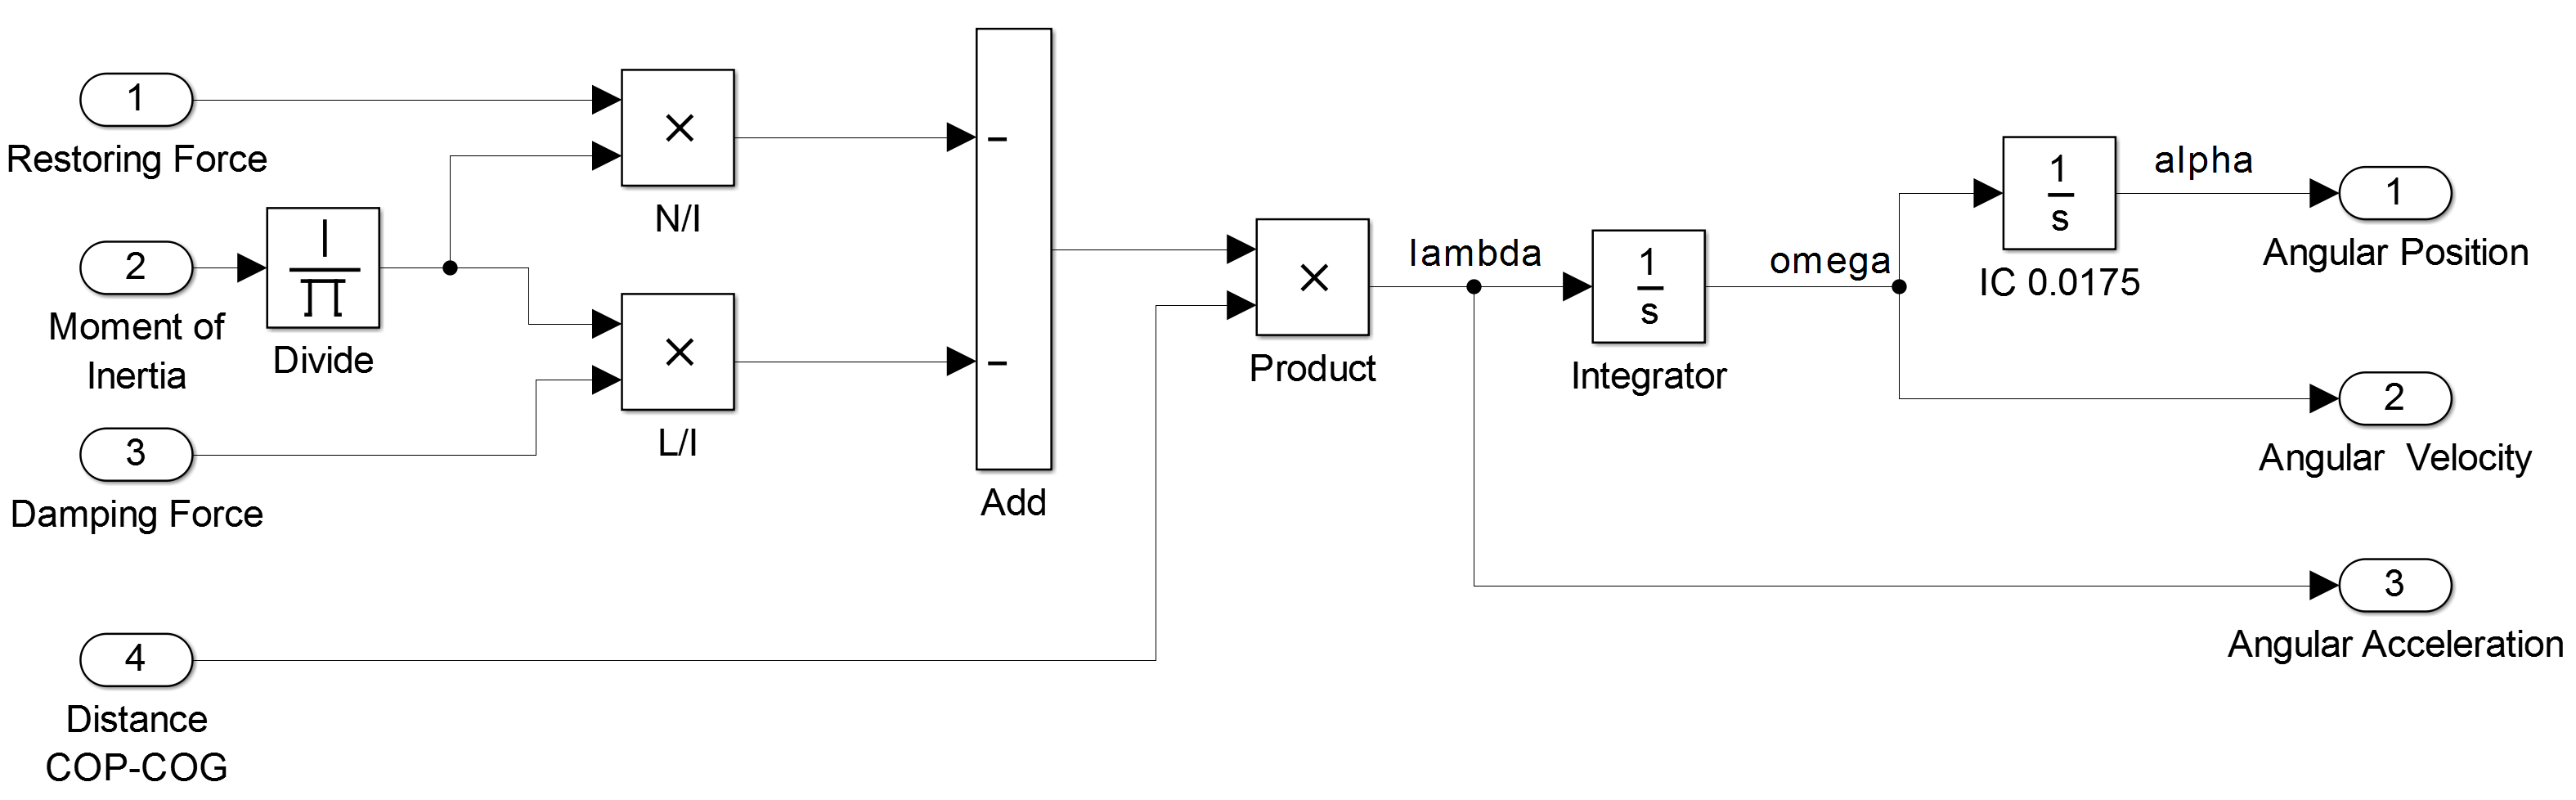
\includegraphics{images/angular_model_simplified.png}
\caption{Angular Flight Model - Simplified
\label{angular_model_simplified}}
\end{figure}

\[
I_L (D^2 - \omega^2) - C_2 D + C_1 = 0
\] \[
-2 I_L D + C_2 = 0
\]

{[}1{]}

A rocket can be considered restored from a disturbance if the angle of
attack decays to 5\% of the initial amplitude {[}1{]}.

{[}1{]}

The \emph{Natural Frequency} of the rocket at the current air speed for
the homogeneous solution is

\begin{equation}
\label{eq_natural_frequency_homogeneous}
\omega_n = \sqrt{ \dfrac{C_1}{I_L} }
\end{equation}

Note: it would appear that this response only reflects the physical
system for non-decreasing values of \(C_2\), which would cause the
exponential term to increase with time and cause the amplitude to grow.
Although the damping coefficient remains relatively constant, the
inverse time-constant is only a function of \(\dfrac{C_2}{2 I_L}\). As
velocity decreases in the rocket coasting phase, \(C_2\) drops
proportional to the square of the velocity and thus the inverse-time
constant decreases enough with respecting time, that \(Dt\) is
decreasing and thus \(e^{-Dt}\) will begin to increase. This is
accounted for by the drift velocity at apogee. While the rocket has a
zero climbing velocity, it does still travel laterally and the total
velocity contributes to the damping moment coefficient, maintaining
stability.

\subsection{Complete Response to Step
Input}\label{complete-response-to-step-input}

\subsection{Complete Response to Impulse
Input}\label{complete-response-to-impulse-input}

\subsubsection{Delta-Dirac Function}\label{delta-dirac-function}

\begin{equation}
\label{eq_delta_dirac}
u(t) = \int_{-\infty}^{\infty} \delta ( u - \tau ) d \tau
\end{equation}

\subsubsection{Convolution Theorem}\label{convolution-theorem}

\subsection{Steady State Response to Sinusoidal
Forcing}\label{steady-state-response-to-sinusoidal-forcing}

\subsubsection{Rocket Damping Ratio}\label{rocket-damping-ratio}

The \emph{Rocket Damping Ratio} is calculated as follows.

\begin{equation}
\label{eq_rocket_damping_ratio}
\zeta = \dfrac{C_2}{2 \cdot \sqrt{C_1 I_L}}
\end{equation}

Where:

\begin{itemize}
\tightlist
\item
  \(C_1\) is the \emph{Corrective Moment Coefficient}
\item
  \(C_2\) is the \emph{Damping Moment Coefficient}
\item
  \(I_L\) is the \emph{Longitudinal Moment of Inertia}
\end{itemize}

{[}1{]}

\paragraph{Underdamped Case}\label{underdamped-case}

\begin{equation}
0 < \dfrac{C_2^2}{4I_L^2} < \dfrac{C_1}{I_l} \
\end{equation}

The fastest response is when \(\zeta = \dfrac{\sqrt{2}}{2}\)

\paragraph{Overdamped Case}\label{overdamped-case}

\begin{equation}
\dfrac{C_2^2}{4I_L^2} > \dfrac{C_1}{I_l} \
\end{equation}

\paragraph{Critically Damped Case}\label{critically-damped-case}

\begin{equation}
\dfrac{C_1}{I_l} = \dfrac{C_2^2}{4I_L^2}
\end{equation}

{[}1{]}

\subsubsection{Rocket Natural Frequency}\label{rocket-natural-frequency}

\begin{equation}
\label{rocket_natrual_frequency}
\omega_n = \sqrt{\dfrac{C_1}{I_L}}
\end{equation}

Where:

\begin{itemize}
\tightlist
\item
  \(C_1\) is the \emph{Corrective Moment Coefficient}
\item
  \(I_L\) is the \emph{Longitudinal Moment of Inertia}
\end{itemize}

{[}1{]}

\subsubsection{Time Constants of the
Response}\label{time-constants-of-the-response}

\subsubsection{Complete response to step
input}\label{complete-response-to-step-input-1}

\subsubsection{Complete response to impulse
input}\label{complete-response-to-impulse-input-1}

{[}1{]}

\subsubsection{AOA as a function of
velocity}\label{aoa-as-a-function-of-velocity}

In order to plot the real system behavior, it may be possible to solve
Equation \ref{eq_rocket_diff} where \(\alpha_x\) is a function of
velocity, and solve for \(\alpha_x\) by twice integrating
\(\ddot{\alpha_x}\).

Since AOA is a function of total velocity through the \emph{Corrective
Moment Coefficient} and the \emph{Damping Moment Coefficient}, it may be
possible to solve the system by differentiating with respect to
velocity, rather than by time.

\[
I \left( \dfrac{d^2\alpha}{dt^2} \right) + F(\alpha) + G \left(\dfrac{d\alpha}{dt} \right) = 0
\]

\[
\dfrac{\delta^2 \alpha_x}{\delta t^2} = \dot{v} = \ddot{x}
\]

\[
\dfrac{\delta \alpha_x}{\delta t} = v = \dot{x}
\]

\[
\dfrac{\delta \alpha_x}{\delta t} = v = \dot{x}
\]

Eventually we get to:

\[
\dfrac{d^2\alpha_x}{dv^2} = ...
\]

\subsubsection{Corrections}\label{corrections}

\paragraph{Compressibility Correction}\label{compressibility-correction}

\emph{Barrowman's Method} neglects compressibility effects, however
these effects cannot be neglected above Mach 0.3.

\subsection{Wind Disturbance}\label{wind-disturbance}

We are interested in the damping ratio of the rocket as it stabilizes
towards \emph{zero angle of attack} in reaction to angular disturbances.

As we consider the rocket to have ideal dimensional accuracy, the main
source of flight disturbance is wind.

\subsubsection{Impulse Disturbance}\label{impulse-disturbance}

We can test the ability of the rocket to stabilize due to an initial
angular disturbance, by applying an initial angle of attack. This
simulates a small gust of wind hitting the rocket just as it takes off.

\subsubsection{Constant Disturbance}\label{constant-disturbance}

We can test the ability of the rocket to stabilize due to a constant
disturbance force, as well as applying an initial \emph{angle of
attack}. This simulates a constant wind force coming from a single
direction. As the density of air goes down with increases altitude, this
assumes that the wind speed picks up at higher altitudes to maintain the
constant wind force.

Alternatively, we could model a constant wind speed of \(8.33 m/s\), and
apply the ISA Model for the density as a function of altitude to
determine the changing wind force as the rocket climbs.

\subsection{More Reading}\label{more-reading}

There are further resources on rocket flight stability here: -
http://www.apogeerockets.com/Tech/Rocket\_Stability

\clearpage

\subsection{Model Referencing}\label{model-referencing}

A high level view of all the test models is in the file
\emph{ANGULAR\_FLIGHT\_TESTING.slx} and is shown in the Model Reference
in Figure \ref{angular_model_reference_label}.

\begin{figure}[htbp]
\centering
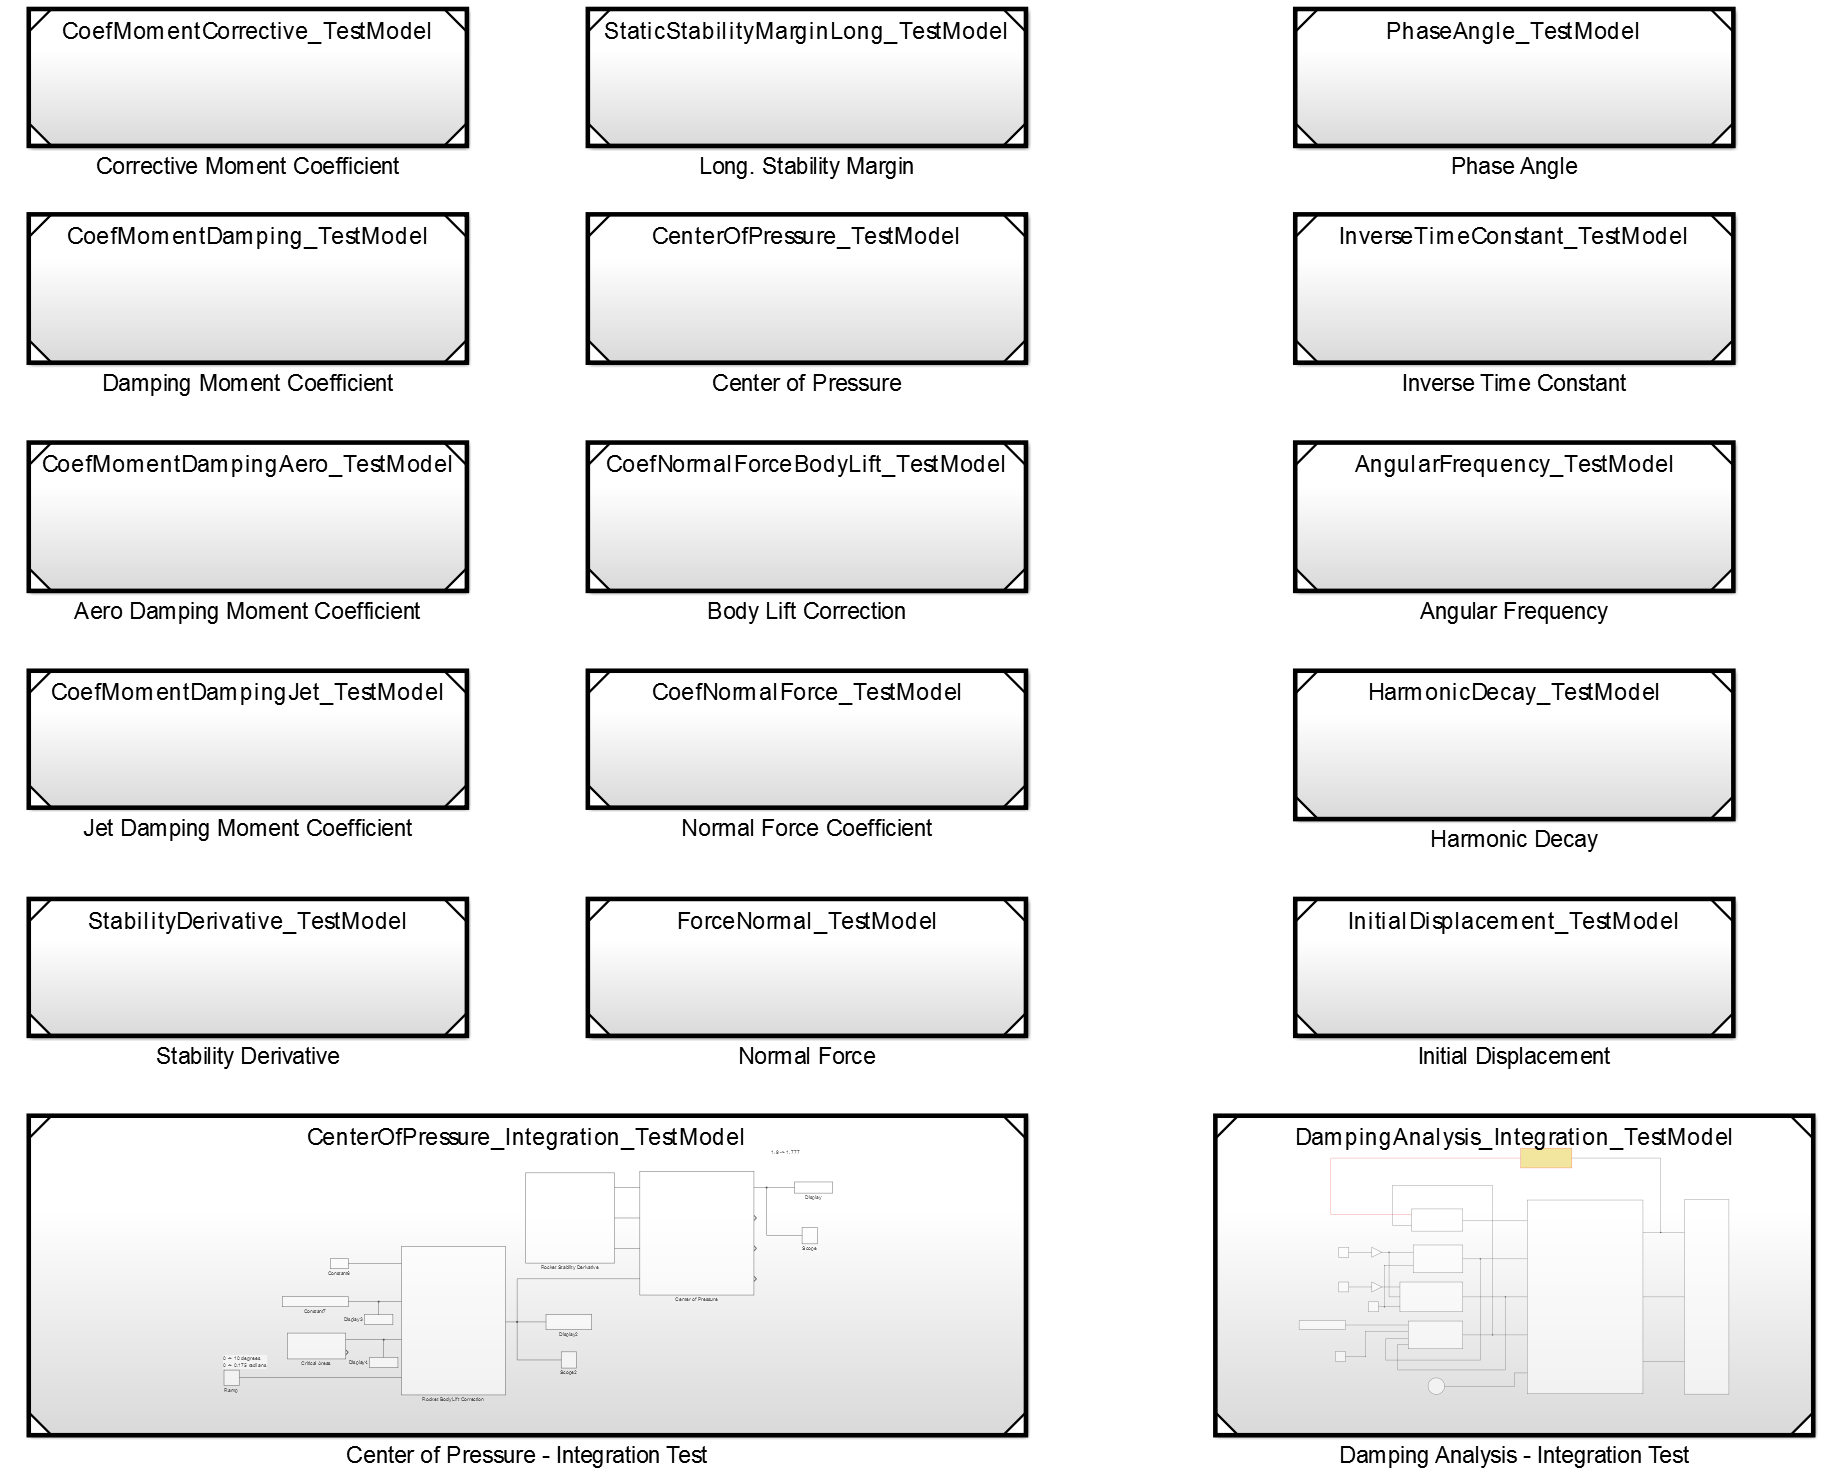
\includegraphics{images/ANGULAR_FLIGHT_TESTING.png}
\caption{Rigid-Body Oscillation - Model Referencing - Simulink
Library\label{angular_model_reference_label}}
\end{figure}

\clearpage

\hyperdef{}{refs}{\label{refs}}
\hyperdef{}{ref-mandell1973}{\label{ref-mandell1973}}
{[}1{]} G. J. C. Mandell Gordon K. and W. P. Bengen., \emph{Topics in
advanced model rocketry}. Cambridge, Mass: MIT Press, 1973.

\hyperdef{}{ref-box2009}{\label{ref-box2009}}
{[}2{]} Simon Box Christopher M. Bishop and H. Hunt, ``Estimating the
dynamic and aerodynamic paramters of passively controlled high power
rockets for flight simulaton,'' February 2009 {[}Online{]}. Available:
\url{http://cambridgerocket.sourceforge.net/AerodynamicCoefficients.pdf}

\hyperdef{}{ref-niskanen2013}{\label{ref-niskanen2013}}
{[}3{]} S. Niskanen, ``OpenRocket technical documentation (development
of an open source model rocket simulation software),'' Master's thesis.

%--------------------------------------------------------------------------------------------------------------
%
%	BACK MATTER
%
%--------------------------------------------------------------------------------------------------------------
%\backmatter

%--------------------------------------------------------------------------------------------------------------
%--------------------------------------------------------------------------------------------------------------
\mainmatter
\end{document}
